        \subsection{sample rate conversion}
	\begin{frame}{sample rate conversion}{introduction}
        \begin{itemize}
            \item   \textbf{applications}
                \begin{itemize}
                    \item   audio file/media conversion
                    \item   word clock synchronization
                    \item   DJing/scratching
                \end{itemize}
            \pause
            \bigskip
            \item   \textbf{terminology}
                \begin{itemize}
                    \item   \textit{synchronous}
                        \begin{itemize}
                            \item   clock rates are coupled
                            \item   resampling factor stays constant
                        \end{itemize}
                    \pause
                    \item   \textit{asynchronous}
                        \begin{itemize}
                            \item   clock rates are independent
                            \item   resampling factor may change
                        \end{itemize}
                \end{itemize}
            \bigskip
            \item   \textbf{ideal result}
                \begin{itemize}
                    \item   spectrum in the used band unchanged
                    \item   periodicity (determined by sample rate) changed
                \end{itemize}
        \end{itemize}
    \end{frame}
	\begin{frame}{sample rate conversion}{introduction}
		\begin{figure}
            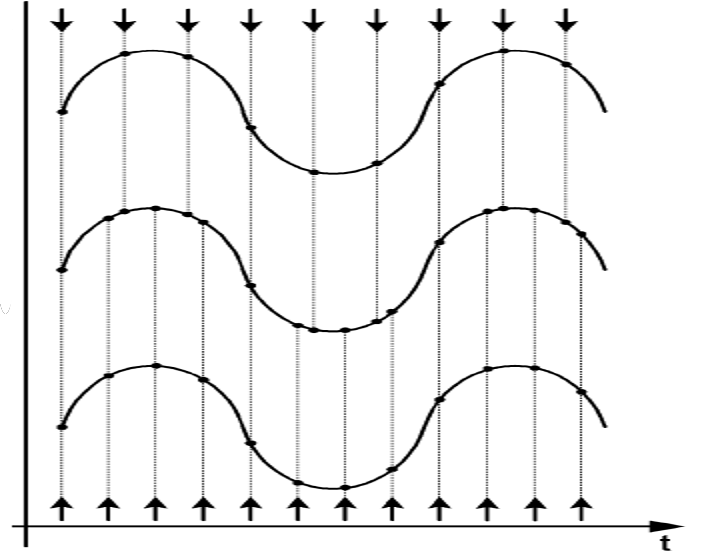
\includegraphics[scale=0.4]{Graph/src_interpolation}
		\end{figure}
    \end{frame}
	\begin{frame}{sample rate conversion}{upsampling by inserting zeros}
        \begin{itemize}
            \item   task: \textbf{upsample by integer factor} $L$
            \pause 
            \begin{enumerate}
                \item   insert $L-1$ zeros between all samples
                \item   apply anti-imaging filter
            \end{enumerate}
        \end{itemize}
        \only<3>{
		\begin{figure}
            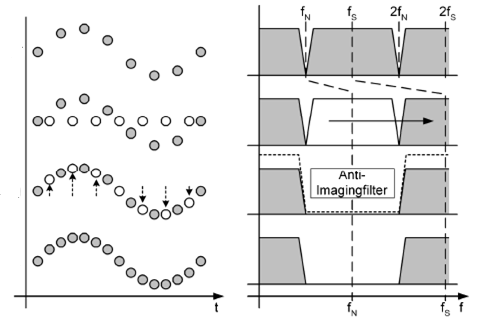
\includegraphics[scale=0.5]{Graph/upsampling}
		\end{figure}
        }
        \only<4>{
		\begin{figure}
            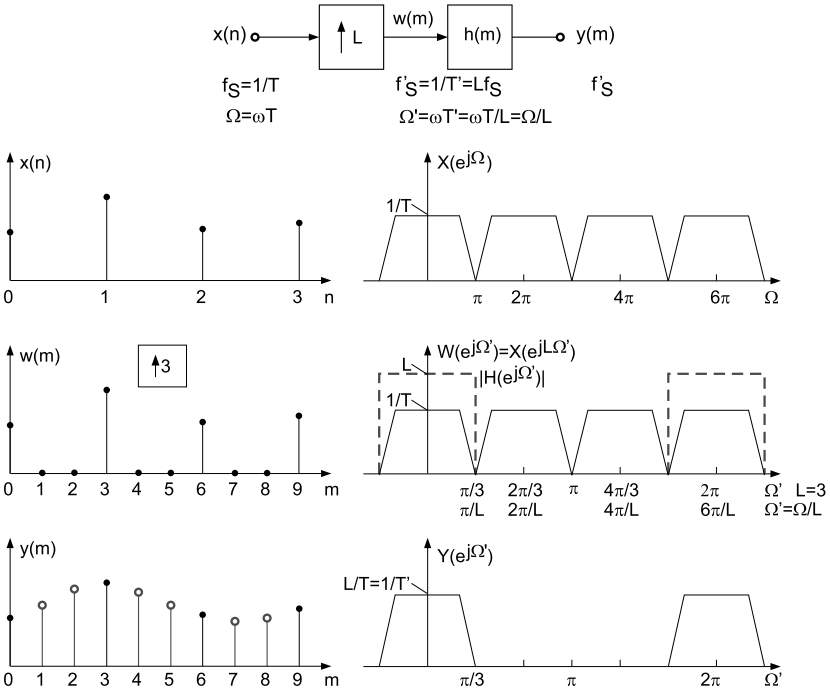
\includegraphics[scale=0.3]{Graph/upsampling_zeros}
		\end{figure}
        }
        \vspace{50mm}
    \end{frame}
	\begin{frame}{sample rate conversion}{downsampling by removing zeros}
        \begin{itemize}
            \item   task: \textbf{downsample by integer factor} $M$
            \pause 
            \begin{enumerate}
                \item   apply anti-aliasing filter
                \item   take every $M$th sample
            \end{enumerate}
        \end{itemize}
        \only<3>{
		\begin{figure}
            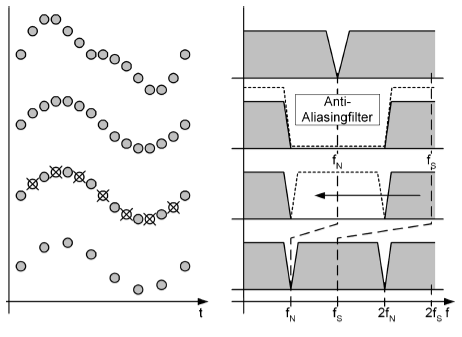
\includegraphics[scale=0.5]{Graph/downsampling}
		\end{figure}
        }
        \only<4>{
		\begin{figure}
            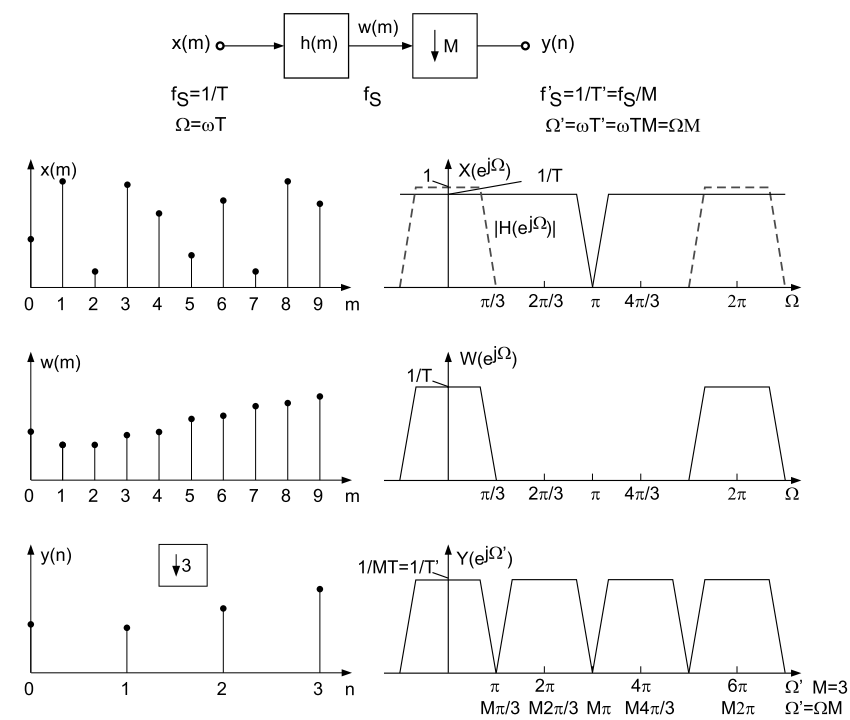
\includegraphics[scale=0.3]{Graph/downsampling_remove}
		\end{figure}
        }
        \vspace{50mm}
    \end{frame}
	\begin{frame}{sample rate conversion}{resampling by rational factor}
        \begin{itemize}
            \item   task: \textbf{convert sample rate to any} other (coupled) sample rate
            \pause 
            \begin{enumerate}
                \item   convert sample rate ratio to integer factors\\ e.g.:  \nicefrac{48}{44.1} $\Rightarrow$ $L=160, M=147$
                \pause
                \item   insert zeros
                \item   apply anti-imaging filter
                \pause
                \item   apply anti-aliasing filter
                \item   remove samples
            \end{enumerate}
        \end{itemize}
        \bigskip
		\only<4->{
        \begin{figure}
            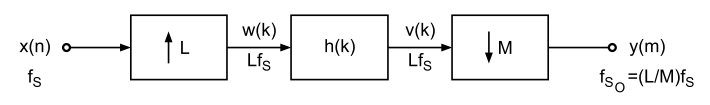
\includegraphics[scale=0.5]{Graph/resampling_flow}
		\end{figure}
        }
        \vspace{50mm}
    \end{frame}
	\begin{frame}{sample rate conversion}{sinc interpolation 1/2}
        \begin{itemize}
            \item   perfect reconstruction of the sampled spectrum is possible with ideal filter
            \item   [$\Rightarrow$] resampling should be possible by time domain convolution with $\sinc$
        \end{itemize}
        \only<1>{
        \begin{figure}
                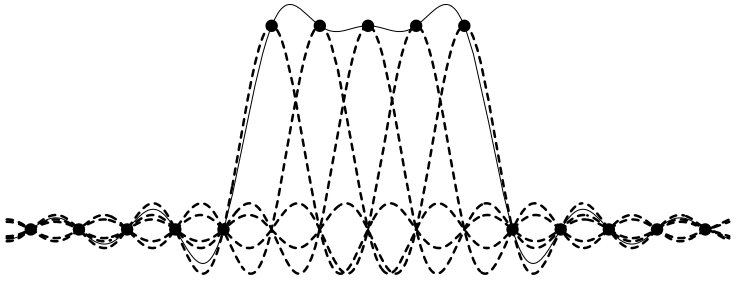
\includegraphics[scale=0.4]{Graph/src_sincinterpol}
        \end{figure}
        }
            \pause
            \begin{equation*}
                x(i-\alpha) = \sum\limits_{m=\-infty}^{\infty}x(m)\frac{\Omega_C}{\pi}\frac{sin\left(\Omega_C(i-\alpha-m)\right)}{\Omega_C(i-\alpha-m)}
            \end{equation*}
            $\Omega_C$ is the cutoff frequency of the  ideal lowpass
        \visible<2>{
        \begin{figure}
                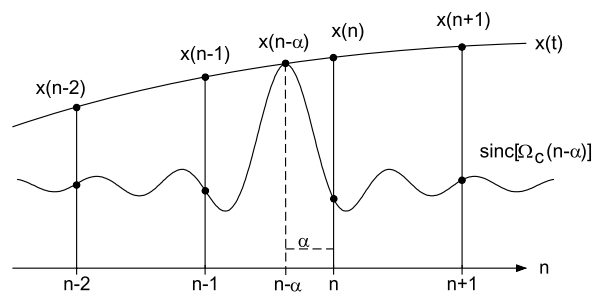
\includegraphics[scale=0.4]{Graph/resample_sinc}
        \end{figure}
        }
    \end{frame}
	\begin{frame}{sample rate conversion}{sinc interpolation 2/2}
        \begin{itemize}
            \item   practical implementation: \textbf{windowed sinc}
        \end{itemize}
    \end{frame}
	\begin{frame}{sample rate conversion}{polynomial interpolation}
        \begin{itemize}
            \item   \textbf{interpolation methods }
                \begin{itemize}
                    \item   can be interpreted as filters with time-variant filter coefficients
                    \item   not based on traditional filter desing methods
                \end{itemize}
            \pause
            \item   polynomial interpolation
                \begin{eqnarray*}
                    f(t) &=& \sum\limits_{k=0}^\mathcal{O}x_k p_k(t)\\
                    p_k(t) &=& \prod\limits_{j=0}^\mathcal{O}\frac{t-t_j}{t_k-t_j}
                \end{eqnarray*}
        \end{itemize}
    \end{frame}
	\begin{frame}{sample rate conversion}{polynomial interpolation example}
        \vspace{-5mm}
        \begin{footnotesize}
        \begin{eqnarray*}
            x(t) &=& \frac{1}{t}\\
            \text{nodes: } t &=& [2, 4, 5]\\
            \pause
            p_0(t) &=& \frac{(t-4)(t-5)}{(2-4)(2-5)} = \frac{(t-4)(t-5)}{6}\\
            p_1(t) &=& \frac{(t-2)(t-5)}{(4-2)(4-5)} = -\frac{(t-2)(t-5)}{2}\\
            p_2(t) &=& \frac{(t-2)(t-4)}{(5-2)(5-4)} = \frac{(t-2)(t-4)}{3}\\
            \pause
             f(t) &=& \sum\limits_{k=0}^\mathcal{O}x_k p_k(t)\\
            \pause
            \Rightarrow f(t) &=& p_0\frac{1}{2}+p_1\frac{1}{4}+p_2\frac{1}{5}\\
            &=& 0.025t^2 - 0.275t + 0.95 .
        \end{eqnarray*}
        \end{footnotesize}
    \end{frame}
	\begin{frame}{sample rate conversion}{polynomial interpolation example}
        \begin{figure}
            \begin{center}
                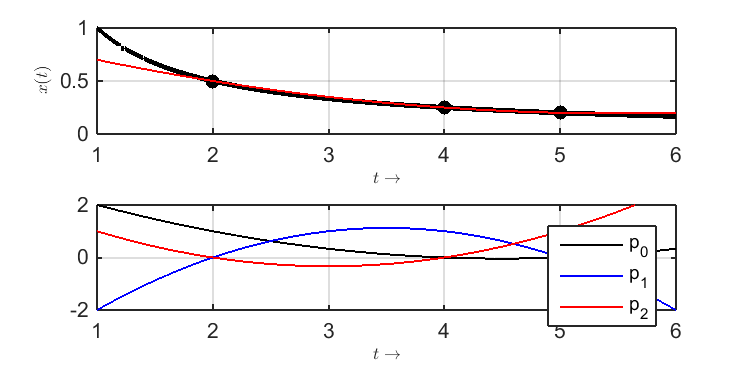
\includegraphics[scale=0.8]{graph/PolynomInterpol}
            \end{center}
        \end{figure}
    \end{frame}
	\begin{frame}{sample rate conversion}{special case: linear interpolation}
        \begin{itemize}
            \item   1st order $\rightarrow$ 2 points
        \end{itemize}
        \begin{footnotesize}
        \begin{eqnarray*}
            x(t) &=& \frac{1}{t}\\
            \text{nodes: } t &=& [2, 4]\\
            \pause
            p_0(t) &=& \frac{(t-4)}{(2-4)} = \frac{(4-t)}{2}\\
            p_1(t) &=& \frac{(t-2)}{(4-2)} = \frac{(t-2)}{2}\\
            \pause
             f(t) &=& \sum\limits_{k=0}^\mathcal{O}x_k p_k(t)\\
            \pause
            \Rightarrow f(t) &=& p_0\frac{1}{2}+p_1\frac{1}{4}\\
            &=& - \frac{1}{8}t + \frac{3}{4}.
        \end{eqnarray*}
         \end{footnotesize}
    \end{frame}
	\begin{frame}{sample rate conversion}{special case: linear interpolation}
        \begin{figure}
            \begin{center}
                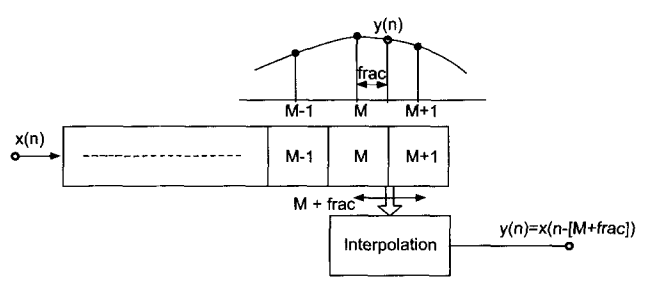
\includegraphics[scale=0.4]{Graph/src_lininterpol}
            \end{center}
        \end{figure}
        
        \begin{equation*}
            \hat{x} = x_l\cdot (1-frac) + x_r\cdot frac
        \end{equation*}
    \end{frame}
	\begin{frame}{sample rate conversion}{interpolation comparison}
        \begin{figure}
            \hspace*{-5mm}
            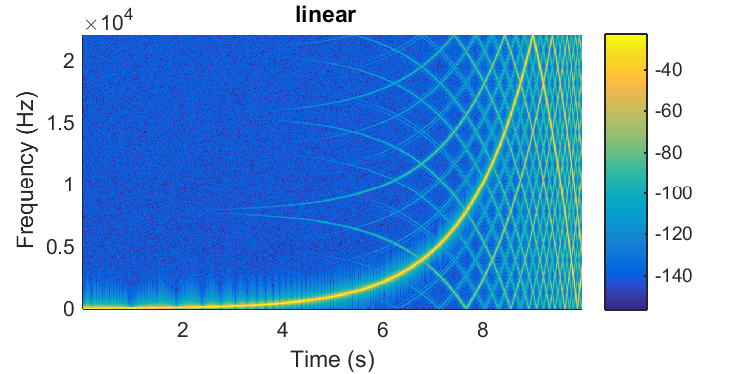
\includegraphics[scale=.5]{graph/src_sine_1}
            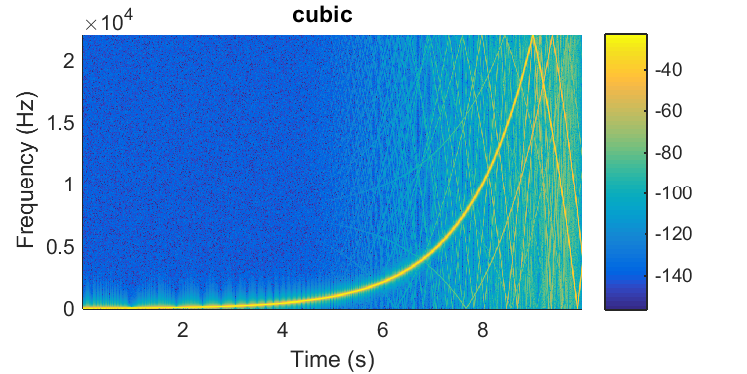
\includegraphics[scale=.5]{graph/src_sine_2}

            \hspace*{-5mm}
            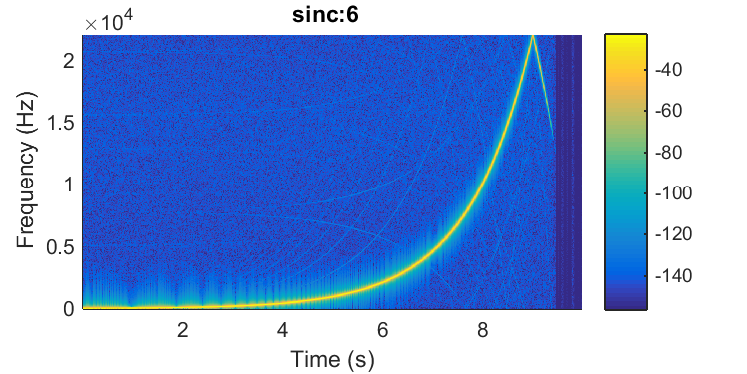
\includegraphics[scale=.5]{graph/src_sine_3}
            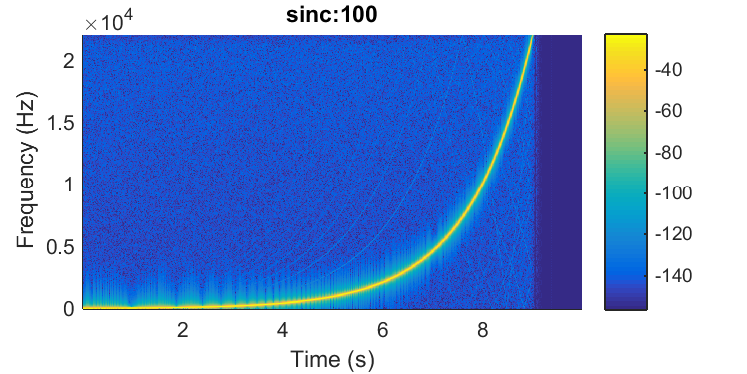
\includegraphics[scale=.5]{graph/src_sine_4}
        \end{figure}
	\end{frame}
	
